\section{PX4 HITL simulation and validation}
\label{sec:test-4-hitl}


This section will delve into the practical implementation of the hardware-in-the-loop (HITL) mode using QGroundControl, Pixhawk 4 board, and the AirSim simulator. The objective is to transition from using a simulated version of the flight stack running on Linux (SITL) to executing the PX4 software natively on a physical Pixhawk board with simulated input and output. This simulation mode allows for real-time testing and validation of the system by integrating physical hardware with simulated environments. 

Achieving a seamless interaction between the simulator, board, and external control applications requires several configuration steps and setting up wired connections. This configuration will be explored to achieve a system that can run the developed control solution, replicating the same behaviour demonstrated in the previous section. In the first part, the DroneVisionControl application will be run from the simulation computer, as outlined in Figure \ref{fig:hitl-connections}. In the second part, after the performance of the flight board is validated, the execution of the DroneVisionControl application will be moved to a separate companion computer, the Raspberry Pi 4. This dual approach allows testing both the offboard and onboard configurations.

\subsection{HITL validation with simulation computer (offboard configuration)}

The purpose of this section is to test the offboard configuration on the ground before any flight tests, with the PX4 flight stack running on the dedicated autopilot board and the DroneVisionControl application running on the simulation computer. To run the flight stack on the Pixhawk board without flying, it is necessary to use the HITL simulation mode, where the flight mechanics will still be simulated by AirSim. The steps for setting up the HITL simulation environment include configuring the flight board through QGroundControl, configuring AirSim to connect to a physical board, and adding new communication channels for additional control mechanisms (DroneVisionControl and RC). QGroundControl provides a specific quadcopter HITL airframe configuration, which initializes the board with all the necessary parameters to activate the simulation mode. The details of these parameters can be found in Appendix \ref{app:install-hitl}. Configuring the board using QGroundControl is a straightforward process. Simply connecting the Pixhawk 4 board to the computer through its debug Micro-USB port will make QGroundControl automatically detect and establish a connection with the board.


On the AirSim side, enabling the simulator to work in HITL mode requires modifying its configuration file. Specifically, the option to accept serial connections needs to be enabled. This file is described in detail in Appendix \ref{app:airsim-config}.
It is important to note that both QGroundControl and AirSim cannot simultaneously establish a connection to the Pixhawk board through the same USB port. Only one of them can be active and connected to the board at any given time. Consequently, QGroundControl must be shut off while conducting the simulation to allow AirSim to establish the necessary communication with the board.


To test the complete system configuration for HITL, as outlined in Figure \ref{fig:hitl-connections}, the Pixhawk board requires an additional communication channel dedicated to the MAVLink exchange with the DroneVisionControl application. This channel is achieved by adding a telemetry radio to the board, which will connect to a counterpart radio on the simulation computer. This wireless link, along with the already existing USB connection, will provide the two separate MAVLink channels needed to complete the environment.
As the AirSim simulator requires a higher update rate compared to the DroneVisionControl application, it is important to keep the Pixhawk to AirSim connection on the wired link. The DroneVisionControl application, on the other hand, sends and receives commands from the Pixhawk at a lower rate, as it depends on the results of the slower computer vision algorithms. The data transmission rate of the radio link is, therefore, sufficient for this application.

Since the flight stack now runs on a physical controller, it becomes possible to attach an RC antenna to the \texttt{PPM RC} port of the board. This antenna allows the vehicle to be flown using an independent RC controller\footnote{\url{https://docs.px4.io/main/en/config/radio.html}}. By configuring the switches in the RC unit for flight mode change or as a kill switch, additional tests can be carried out to verify the developed safety features described in Section \ref{subsec:safety}, like interrupting autonomous flight upon flight mode changes or upon loss of signal from the RC controller.


After all the necessary connections are set up and the AirSim simulator started, the control program can be started with the following command:
\begin{minted}[breaklines, fontsize=\footnotesize, baselinestretch=1]{bash}
dronevisioncontrol follow --sim --serial COM[X]:57600
\end{minted}
The \texttt{COM[X]:57600} section describes the serial connection to the telemetry radio, where the COM port number will vary depending on the particular USB port to which the telemetry radio is connected, and the baudrate specified is 57600.



\subsection{HITL validation with Raspberry Pi (onboard configuration)}
\label{sec:test-5-rpi}

\begin{figure}[H]
  \centering
  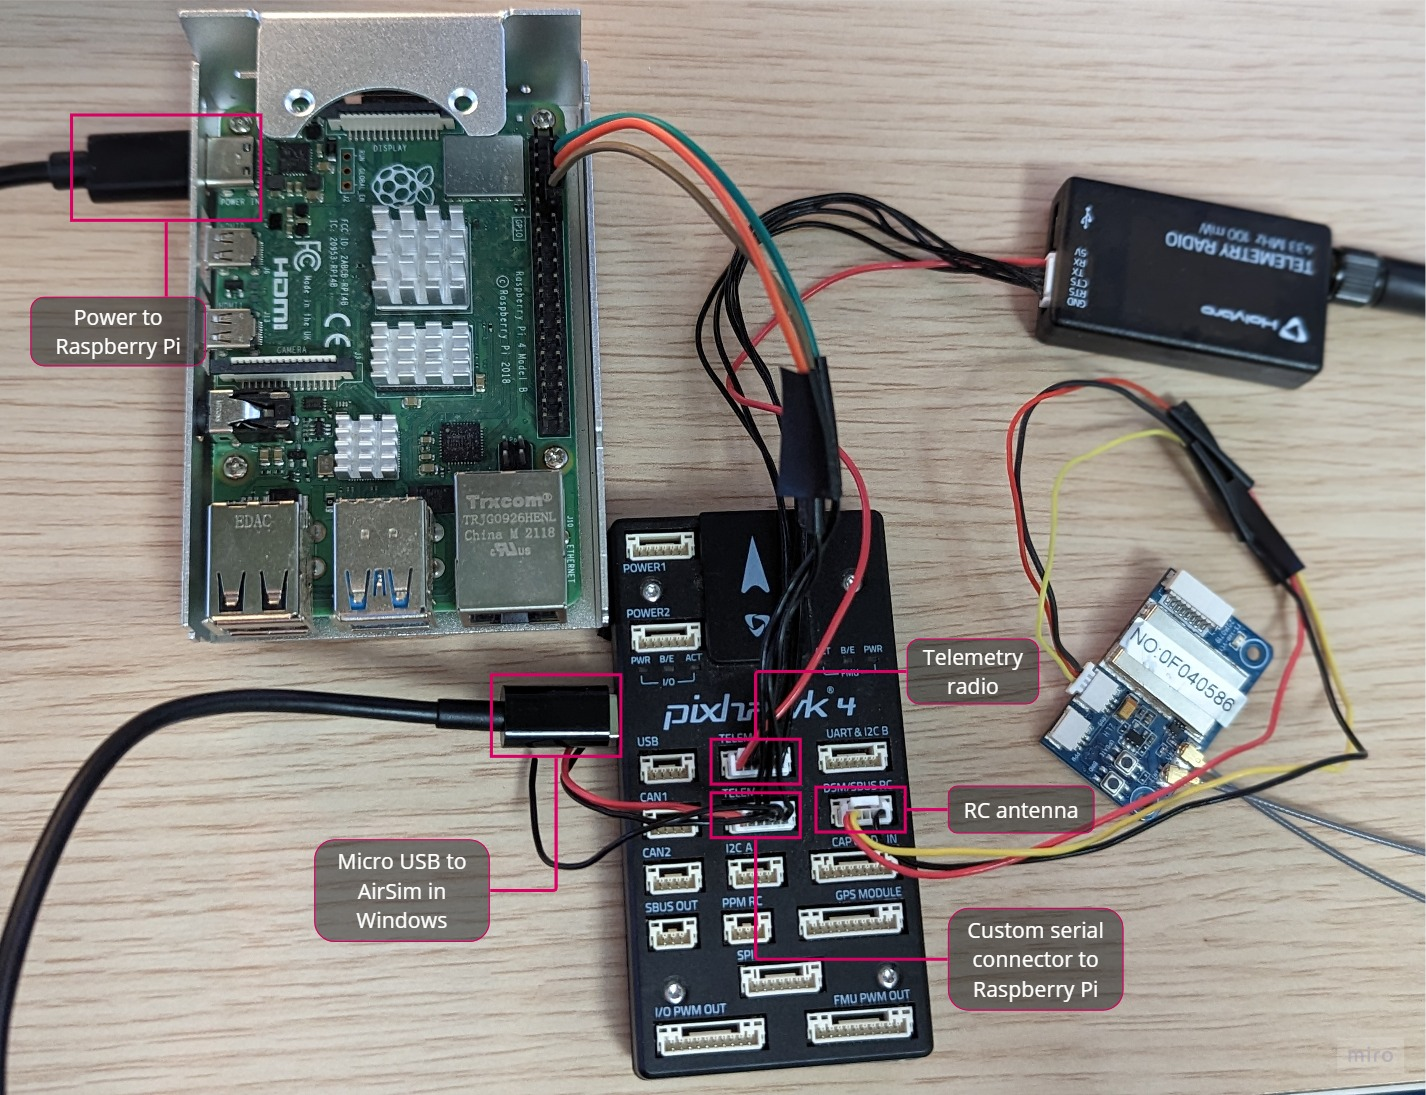
\includegraphics[width=\textwidth, keepaspectratio]{img/hitl-setup-picture.jpg}
  \caption{Pixhawk 4 board connected to a Raspberry Pi running the DroneVisionControl application and a Windows computer running the AirSim simulator. The setup includes a telemetry radio for QGroundControl and an RC receiver for manual control.}
  \label{fig:hitl-setup-picture}
\end{figure}

The next crucial step in transitioning from a fully simulated environment to real flight is to establish a connection between the future onboard computer, the Raspberry Pi 4, and the Pixhawk flight controller. This connection enables conducting more realistic tests using the same hardware as during flight tests to allow the identification of potential hardware performance issues. The tests mimic the onboard computer configuration outlined in Figure \ref{fig:onboard-config}, with the DroneVisionControl application running on an onboard companion computer.

Figure \ref{fig:hitl-setup-picture} provides an overview of the connections used for HITL testing with the Raspberry Pi. The main addition from the previous section is the direct connection between the Pixhawk board and the Raspberry Pi's I/O pins. While the inclusion of the telemetry radio is not strictly required in this scenario, it enables maintaining a simultaneous connection to QGroundControl on the ground station or simulation computer, facilitating better oversight and monitoring.

Before any tests can begin, the operating system of the Raspberry needs to be set up for the DroneVisionControl application. A detailed explanation of the complete installation process, along with all the necessary libraries and dependencies for the Raspberry Pi, is included in Appendix \ref{app:install-hitl}. To conveniently control the Raspberry Pi during the installation, a remote desktop connection is recommended. This allows for transmitting screen contents, as well as mouse and keyboard input, over a local network. Thus, accessing the Pi's desktop from the ground station computer becomes feasible, even during flight. One available option to achieve this is XRDP\footnote{\url{http://xrdp.org/}}, an open-source implementation of a Microsoft Remote Desktop Protocol server that is compatible with the Raspberry OS.

To ensure successful progress towards autonomous flight, several key characteristics of the Raspberry Pi must be addressed:
\begin{enumerate}
    \item Power supply. Capacity to function when powered by a battery.
    \item Serial connection. Pixhawk to Raspberry Pi and Pixhawk to the simulation computer.
    \item DroneVisionControl software. Ability to run the DroneVisionControl application and its dependencies.
    \item Performance of computer vision algorithms with limited processing power.
\end{enumerate}


\subsubsection{Verify power supply}

The first step is to verify that the Raspberry Pi can be powered by a secondary battery connected to the board's power port by a USB-C cable instead of the standard AC power supply. Through this battery, sufficient power must be provided to the Raspberry Pi to maintain enough processing speed for the image processing software and to power the camera connected to the board. The performance differences between powering the Raspberry board with the AC supply and the battery are detailed in Section \ref{subsec:performance}. At this point, it is enough to check that the \texttt{test-camera} utility can run at an acceptable frame rate with either hand or pose detection enabled on previously recorded images from the camera or simulator.


\subsubsection{Verify serial connections}

The most important connection that needs to be verified is the MAVLink communication channel between the flight controller and the onboard computer. The custom connector described in Table \ref{tab:wiring-telem} is used for this purpose, with the \texttt{TELEM2} port on the Pixhawk board connected to the TX/RX UART pins on the Raspberry Pi's GPIO header. Additionally, configuration is required for the flight controller and the companion computer. For the PX4 flight controller, only the \texttt{TELEM1} port of the Pixhawk is configured for telemetry radio. An additional MAVLink channel must be configured in QGroundControl by setting the correct values to the parameters listed in \ref{tab:telem2-params}.
On the Raspberry Pi side, the serial port is configured by default to exchange shell messages. This needs to be disabled using the \texttt{raspi-config} command-line utility and selecting the following steps: Interface options -> Serial Port -> Disable login shell, enable serial port hardware (see Figure \ref{fig:serial-connection}). After making these changes, the \texttt{/dev/serial0} address can be used to communicate with the device at the baud rate configured in QGroundControl.

The remaining connections serve to communicate the Pixhawk board and the simulation computer. Two different channels are needed to be able to exchange information with QGroundControl and AirSim at the same time. The connection to AirSim will be implemented through the development-only micro-USB port on the Pixhawk board, and the connection to QGroundControl through the telemetry radio. Due to the substantially lower throughput of the telemetry radio in comparison with the USB cable, using the telemetry radio to communicate between the Pixhawk board and AirSim will result in inferior performance since there is a more significant amount of messages transferred than between QGroundControl and the Pixhawk.

\begin{table}[h!]
 \begin{center}
  \begin{tabular}{l|l}
    Parameter name & Value \\ \hline
    MAV\_1\_CONFIG & TELEM2 \\
    SER\_TEL2\_BAUD & 921600 \\
  \end{tabular}
  \caption{PX4 parameters that require configuration to enable MAVLink communication through the secondary telemetry port.}
  \label{tab:telem2-params}
 \end{center}
\end{table}


\begin{figure}
  \centering
  \makebox[\textwidth][c]{
  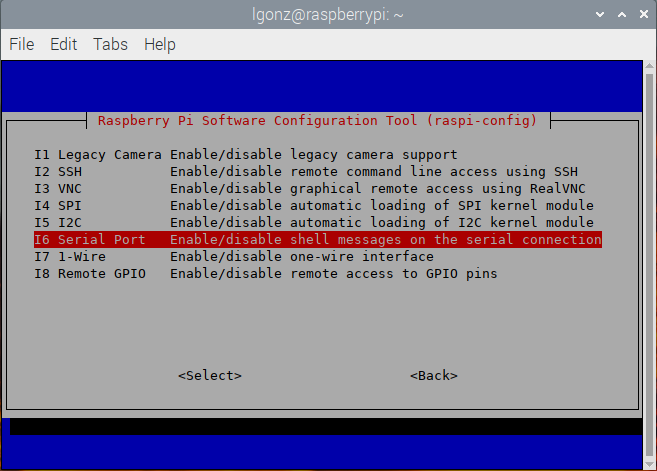
\includegraphics[width=.615\textwidth, keepaspectratio]{img/raspi-config.png}
  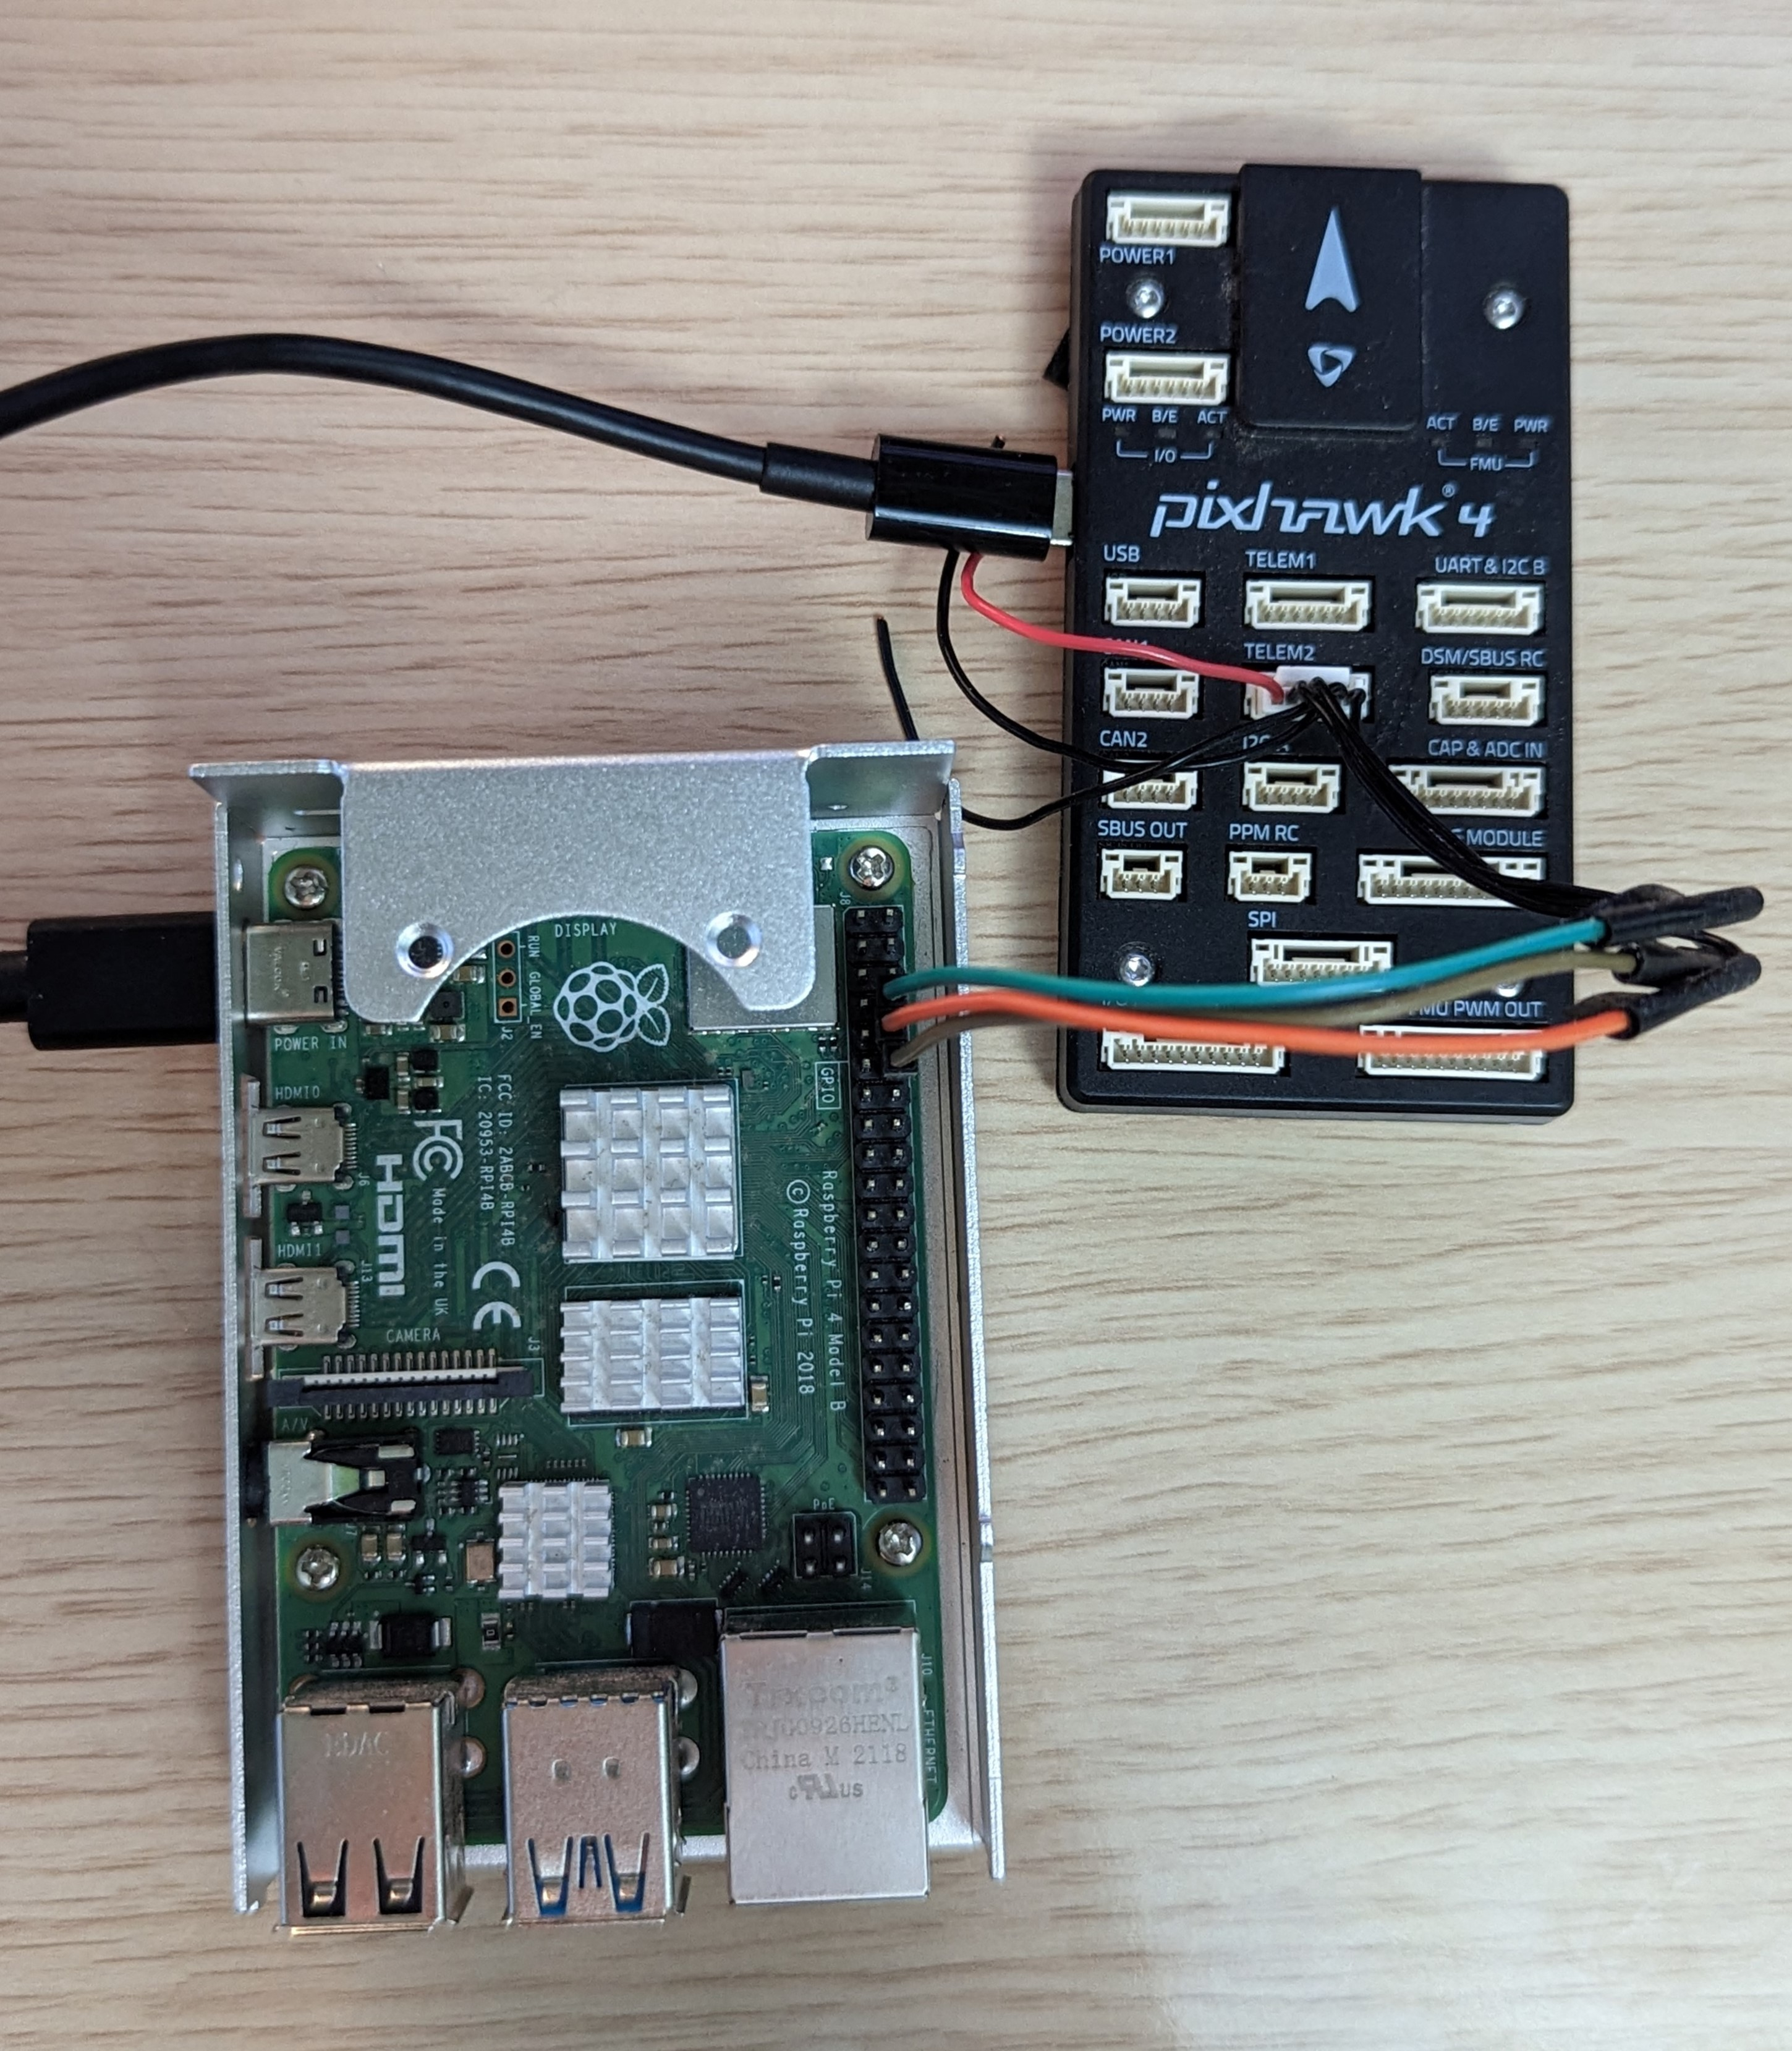
\includegraphics[width=.385\textwidth, keepaspectratio]{img/rpi-pixhawk-serial.jpg}}
  \caption{a) Picture of Raspberry's \texttt{raspi-config} and b) close-up of Pixhawk to Pi cable connection.}
  \label{fig:serial-connection}
\end{figure}


\subsubsection{Verify DroneVisionControl software}

To validate the complete configuration, the test camera utility will be used by executing the following command in the Raspberry Pi:

\begin{minted}[breaklines, fontsize=\footnotesize, baselinestretch=1]{bash}
dronevisioncontrol tools test-camera --hardware /dev/serial0:921600 --sim <AirSim host IP> --pose-detection
\end{minted}

This command connects DroneVisionControl to PX4 via the hardware address \texttt{/dev/serial0} at a baudrate of 921600. Meanwhile, the images from the simulator's virtual camera are sent to the Raspberry Pi over the local area network. The \texttt{<AirSim host IP>} parameter defines the IP the application will connect to to receive these images.

The result from the execution is shown in Figure \ref{fig:rpi-airsim-test}. On the right side, the remote connection to the Raspberry Pi's desktop is displayed, showing the output of the DroneVisionControl program running the pose detection algorithm on the images received from the simulator. On the left side of the figure, the AirSim simulator renders the movements of the vehicle as it responds to the instructions from the flight controller that listens to the companion computer.

\begin{figure}
  \centering
  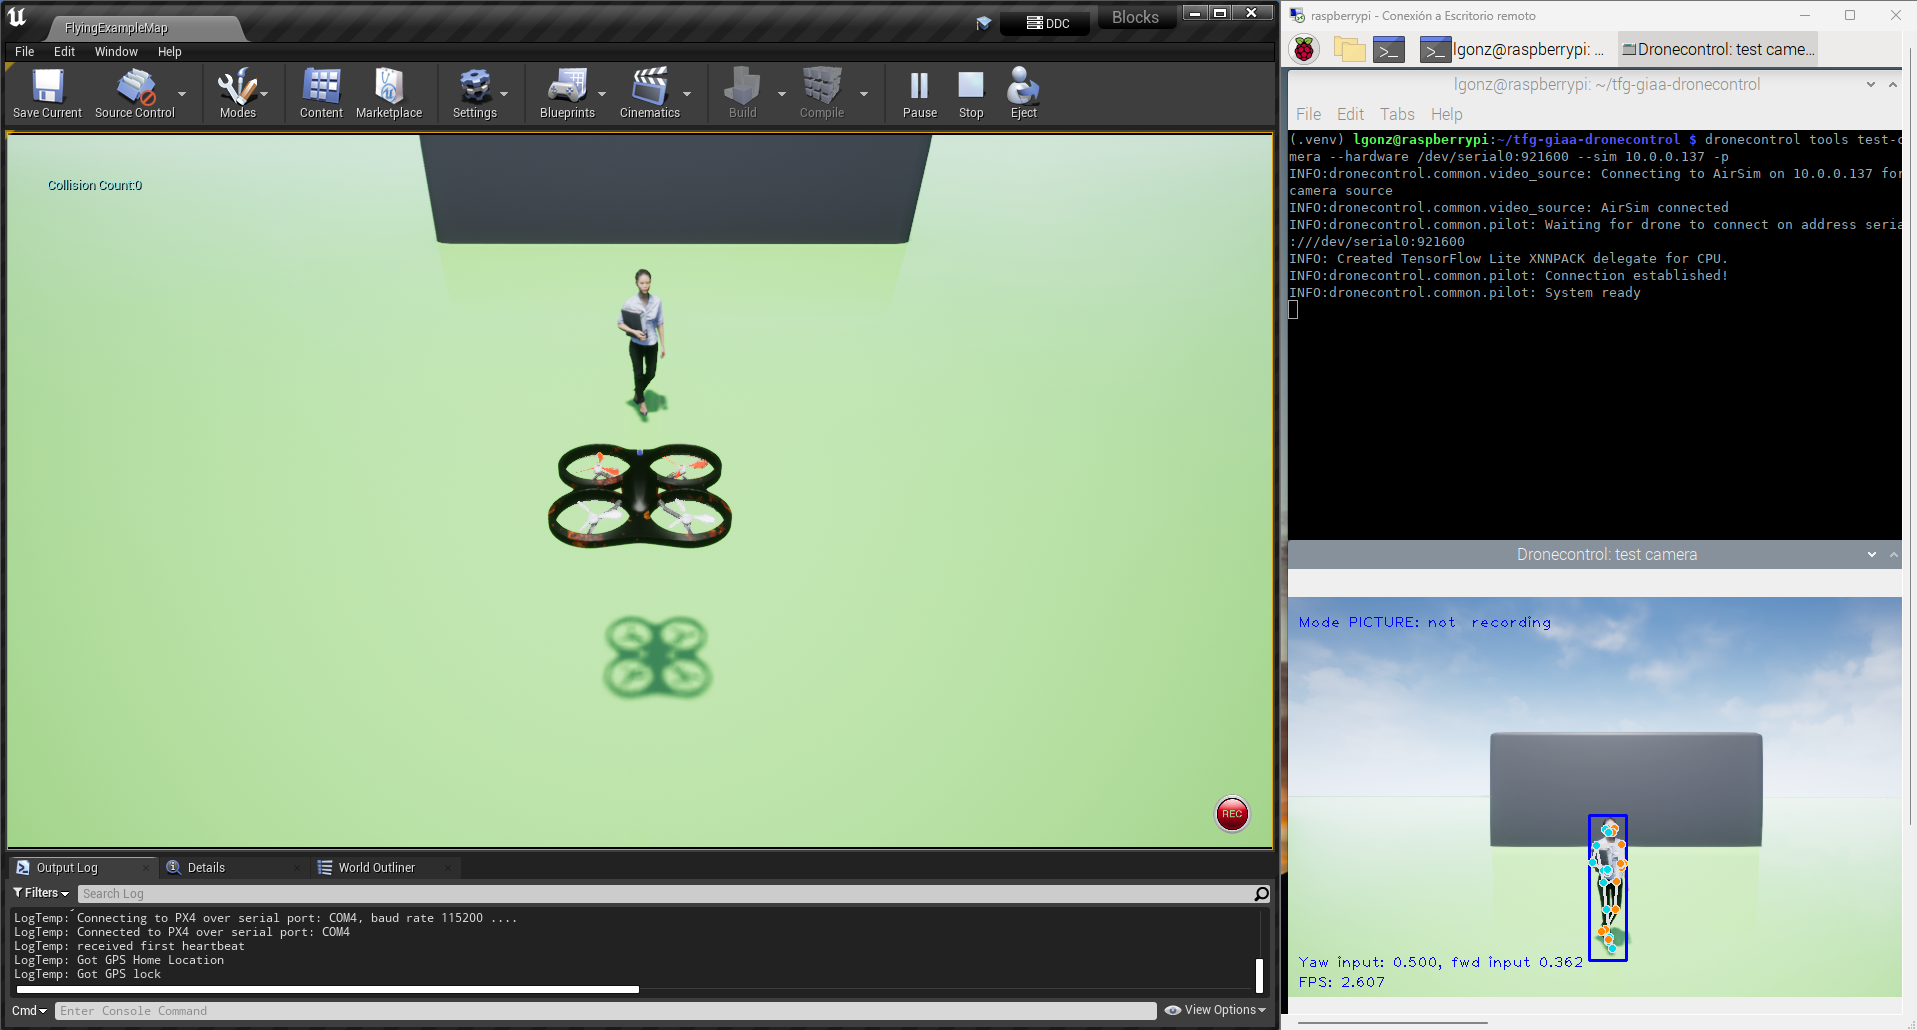
\includegraphics[width=\textwidth, keepaspectratio]{img/airsim-rpi-test.png}
  \caption{Left: AirSim simulator on Windows host. Right: RPi desktop with DroneVisionControl application and pose output.}
  \label{fig:rpi-airsim-test}
\end{figure}


\subsection{Performance analysis}
\label{subsec:performance}

One crucial question that remains to be answered before the vehicle can take flight using this hardware and software configuration is whether the Raspberry Pi 4b's modest processor, a quad-core ARM Cortex-A72 64-bit SoC running at 1.5GHz, can handle the detection and tracking algorithms with sufficient performance and respond effectively to real-time movement. To address this matter, the average time spent by the program on each task in the running loop can be calculated and analyzed under different scenarios. This analysis will help estimate the maximum speed at which the algorithm can track a person.


Based on the running loop for the follow solution described in Section \ref{sec:follow} and shown in Figure \ref{fig:follow-loop}, the processing cost can be divided into several distinct areas that can be measured independently: image processing, offboard control, manual input, and released thread (overhead from the async execution). Figure \ref{fig:perf-sitl-sim} illustrates the time allocation for each task during an average run of the follow solution with PX4 running in SITL mode and AirSim as the simulator. DroneVisionControl was also run on the simulation computer. The time consumption was obtained by measuring the time at the start and end of each task, calculating the time difference between them and averaging across every iteration of the main loop. The utility for this process can be found in the measure function inside the application's utils module\footnote{\url{https://github.com/l-gonz/tfg-giaa-dronecontrol/blob/main/dronecontrol/common/utils.py}}.

\begin{figure}[H]
  \centering
  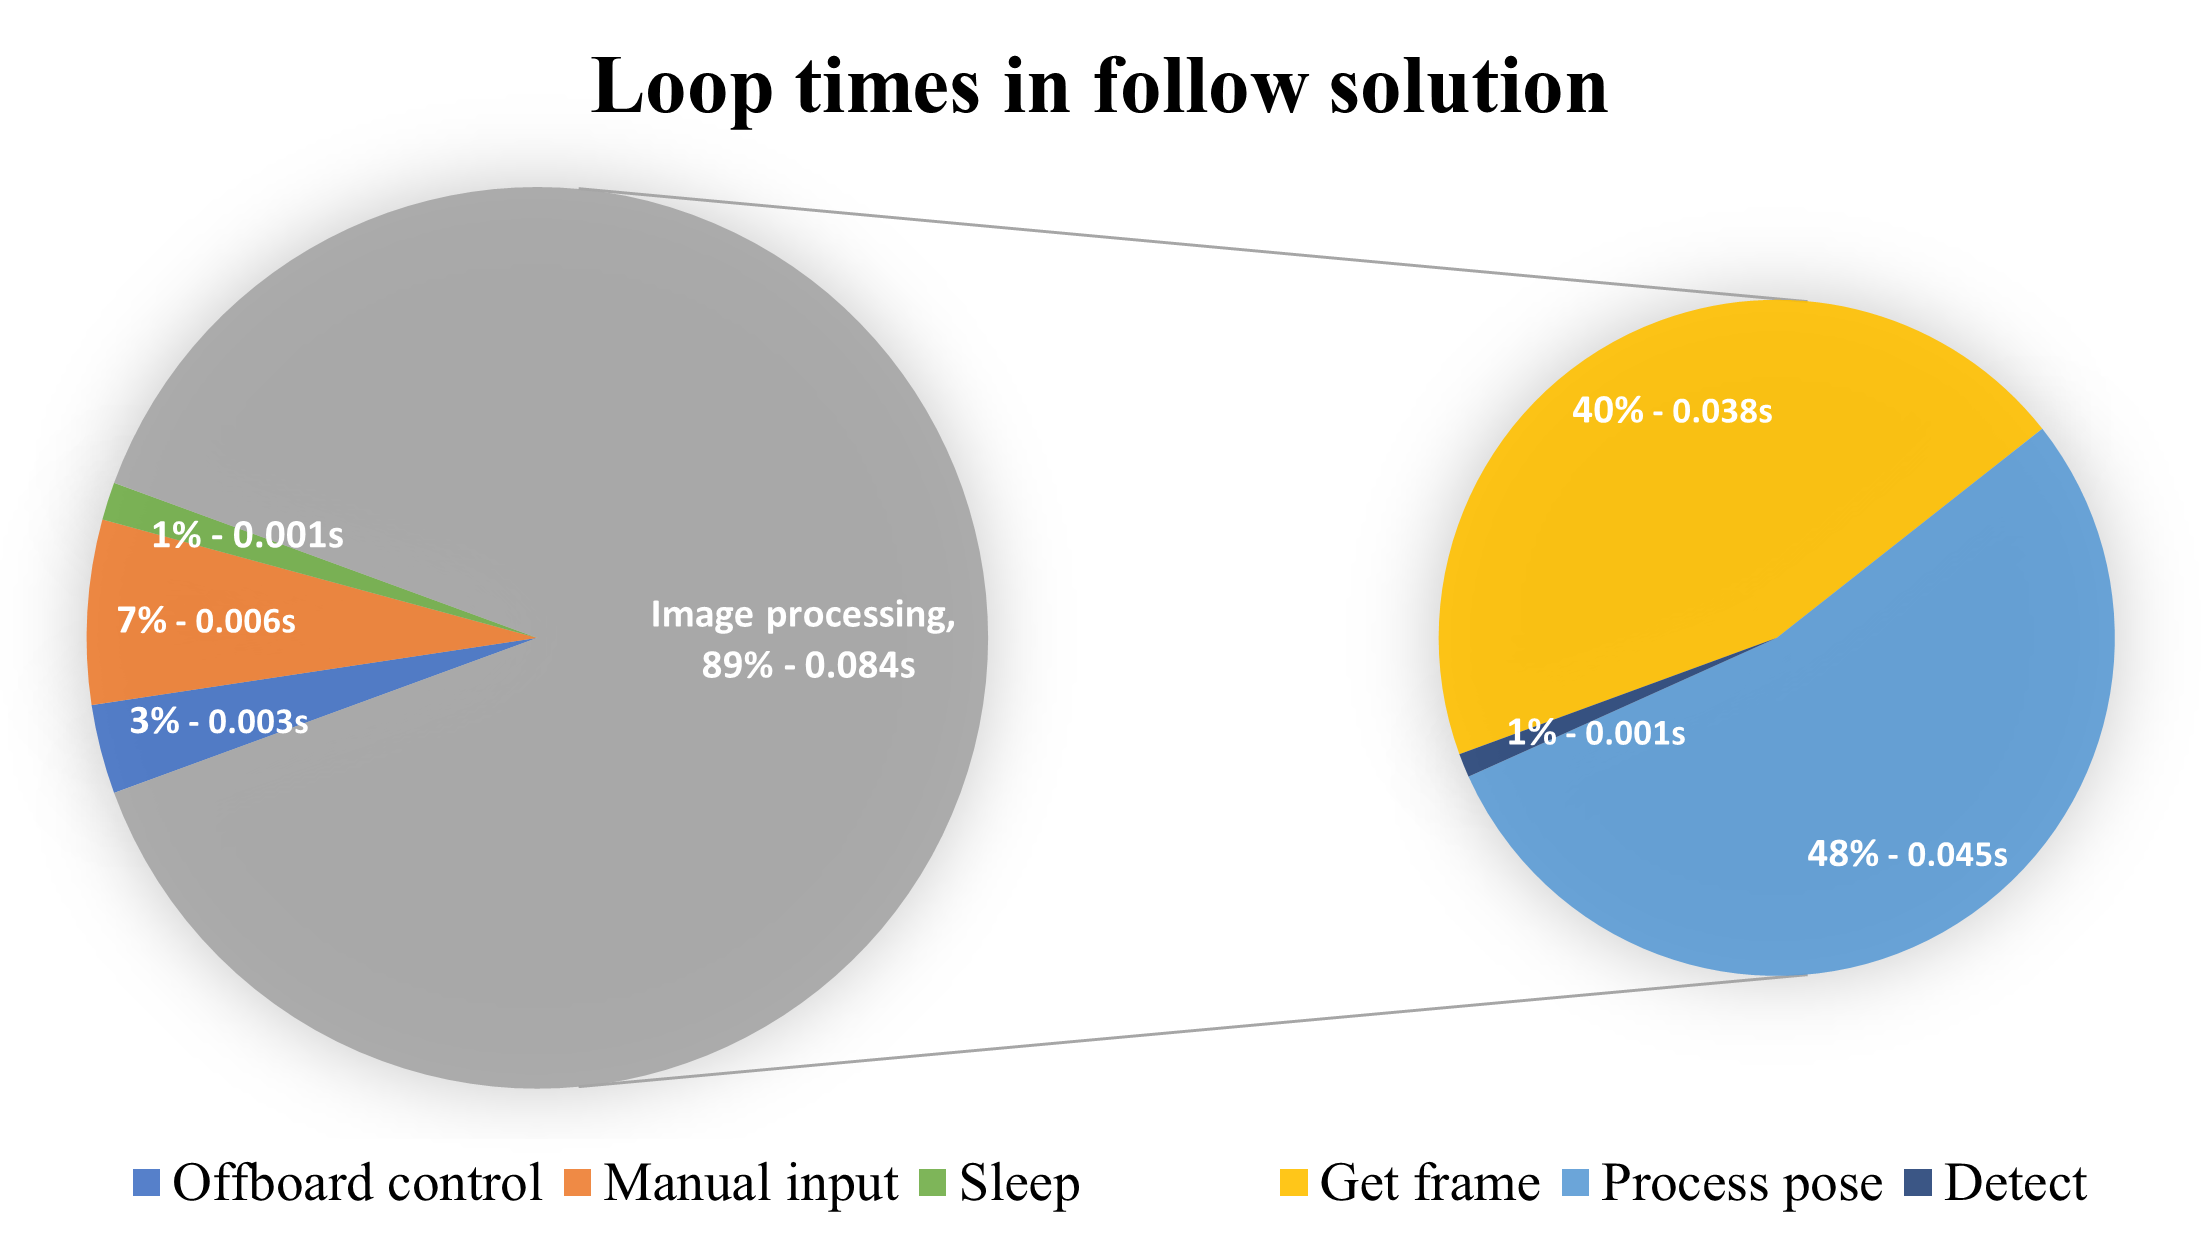
\includegraphics[width=.9\textwidth, keepaspectratio]{img/sitl-performance.png}
  \caption{Average percentages of a loop spent by each task in the follow solution with their corresponding average absolute times in seconds (SITL + AirSim configuration).}
  \label{fig:perf-sitl-sim}
\end{figure}


The most time-consuming task is image processing, which accounts for approximately 89\% of the total loop time. To gain further insight into the time allocation within the image processing task, the work can be further divided into three subtasks:
\begin{enumerate}
    \item \textbf{Get frame}, which involves requesting a new frame from the video source.
    \item \textbf{Process pose}, which entails sending the frame to the MediaPipe library for detection and tracking.
    \item \textbf{Detect}, which involves calculating the bounding box coordinates and determining whether it represents a valid pose.
\end{enumerate}

As shown in \ref{fig:perf-sitl-sim} (right), the subtasks take 40\%, 48\%, and 1\% of the total loop time, respectively. The average time for each iteration of the loop is 0.095 seconds, resulting in an average performance of 10.5 \acrfull{fps}.

Similar measurements were conducted for different hardware combinations, employing varying degrees of simulation while running the follow solution in offboard mode and connected to the AirSim simulator. The hardware combinations tested include:
\begin{enumerate}
    \item All simulated hardware: PX4 in SITL mode + DroneVisionControl on the simulation computer + images from the AirSim simulator as the video source.
    \item Simulated hardware with real images: PX4 in SITL mode + DroneVisionControl on the simulation computer + images from an attached camera as the video source.
    \item Test hardware with AC power supply: PX4 in HITL mode on Pixhawk 4 + DroneVisionControl on Raspberry Pi powered by AC + images from an attached camera as the video source.
    \item Test hardware with battery: PX4 in HITL mode on Pixhawk 4 + DroneVisionControl on Raspberry Pi powered by a battery + images from an attached camera as the video source.
\end{enumerate}


\begin{figure}
  \centering
  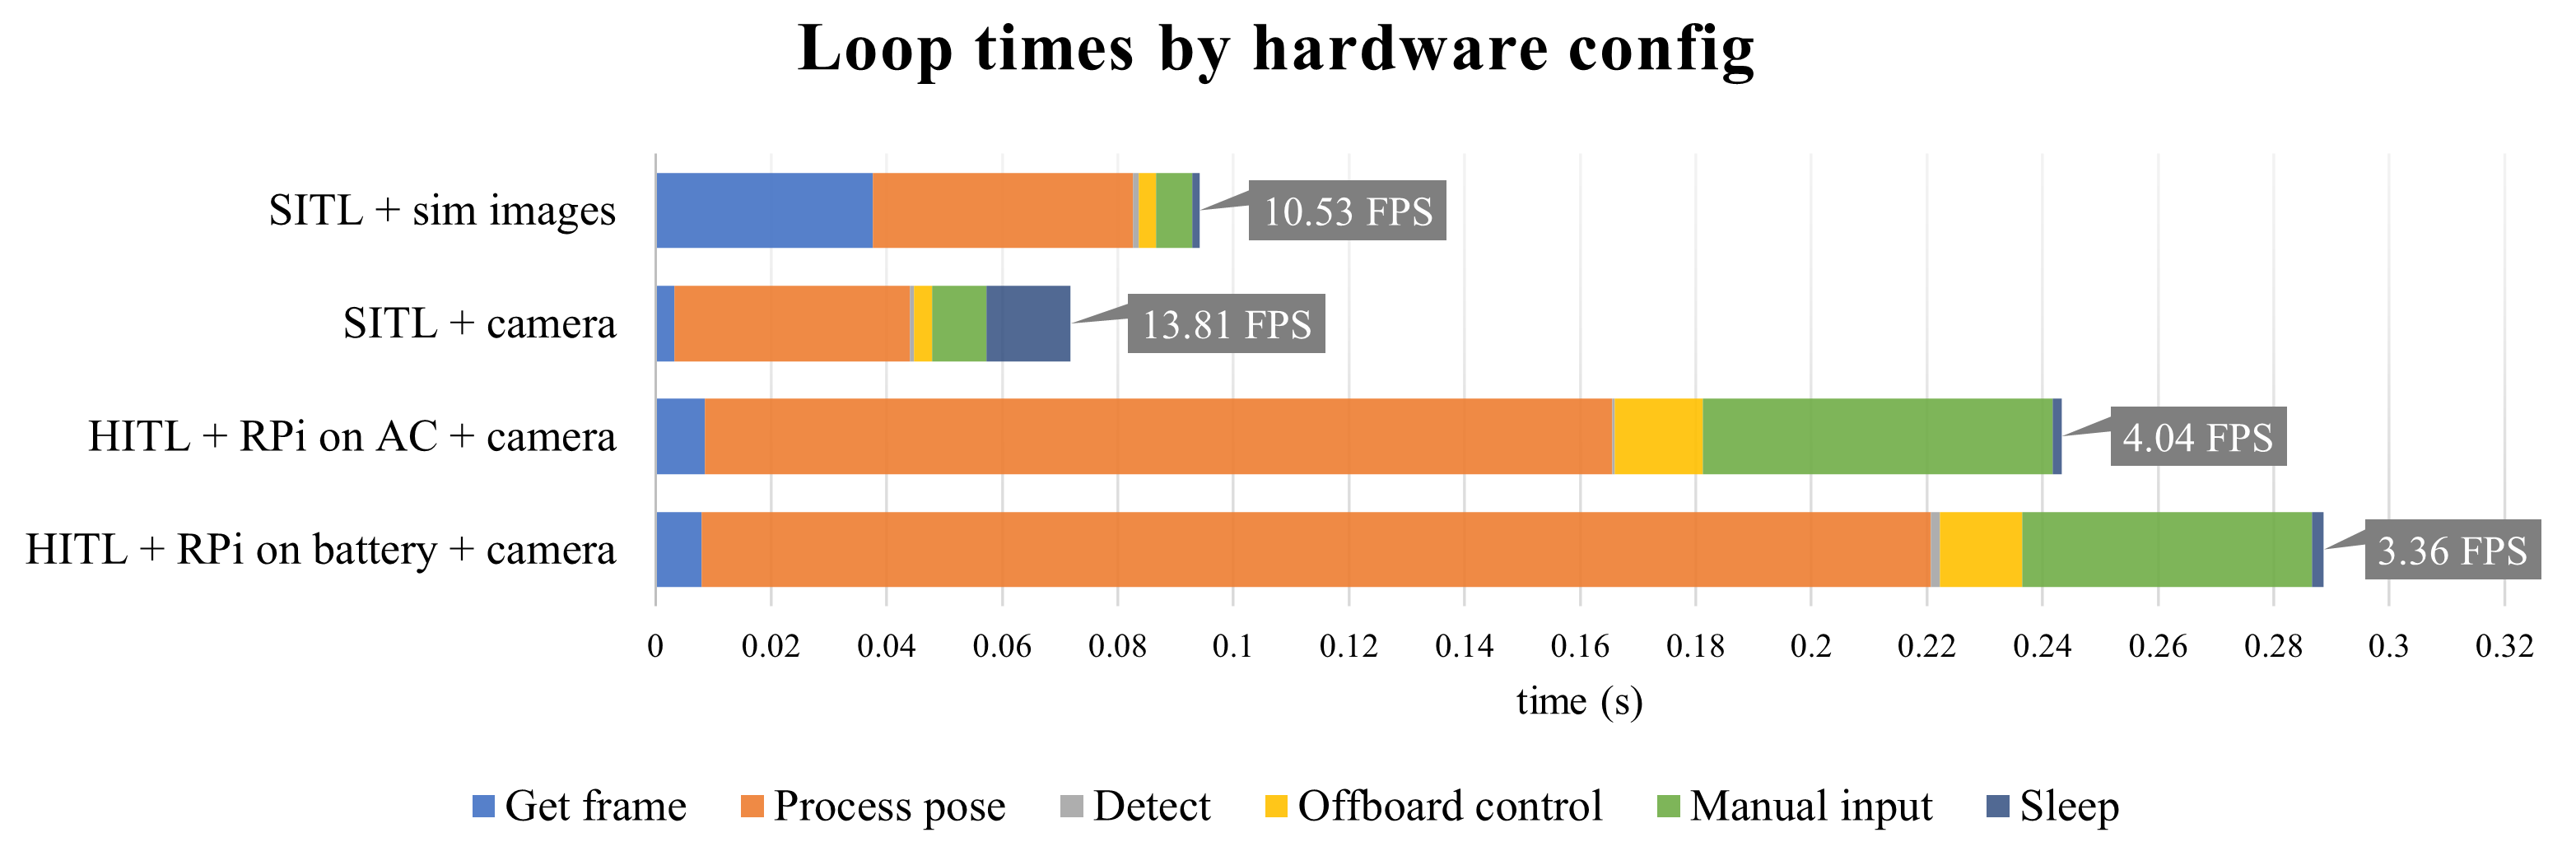
\includegraphics[width=\textwidth, keepaspectratio]{img/performance-graph.png}
  \caption{Average FPS and time spent on each task per iteration of the follow solution for the different hardware configurations.}
  \label{fig:perf-analysis}
\end{figure}


Figure \ref{fig:perf-analysis} presents the average measurements obtained for all the analyzed hardware combinations. In the first test, it is observed that retrieving each new frame from the AirSim simulator takes significantly more time compared to using an external camera. This discrepancy arises from performance limitations in the simulation running on Unreal Engine, which will not be a factor once the simulation engine is no longer used. In the second test, replacing the simulator images with the feed from an external camera results in faster image retrieval and the highest performance among all the tests, averaging 14 FPS with peaks exceeding 20 FPS.

In the third and fourth tests, the image processing calculations are performed on the onboard Raspberry Pi computer, leading to a 400\% to 500\% increase in the time required for pose processing. Additionally, there is also a noticeable difference in performance observed for the Raspberry's processor between powering the computer through the AC power supply and through an external battery. This difference stems from the fact that the former supplies 3A of current to the board and the latter only 2A.

These measurements provide insights into the board's expected behaviour during actual flights, with the fourth test (hardware with battery) representing the closest approximation to real flight conditions. From the results, it is expected that a performance of approximately 3 FPS can be sustained during flight, which gives a time between frames of approximately 0.3 seconds. Considering that the camera's field of view for flight tests covers approximately four meters at the target follow distance, the person being tracked should be able to move at a speed of 3-4 m/s with the drone maintaining line of sight. This performance is satisfactory enough for this project, but there is room for improvement by, for example, optimizing the image processing algorithm or using more powerful hardware for the onboard companion computer.
